%%%%%%%%%%%%%%%%%%%%%%%%%%%%%%%%%%%%%%
%
% This is how you write code:
%
% \begin{minted}{matlab}
% foo = [2 1 0;1 4 3;2 4.5 6];
% \end{minted}
%

% This is how you import code:
% 
% \inputminted[linenos]{matlab}{foo_bar.m}
%
 
% (Most) figures are imported this way:
%
% \begin{figure}
% \includegraphics[width=\textwidth]{foo_figure}
% \caption{This is a caption}
% \end{figure}
%
%%%%%%%%%%%%%%%%%%%%%%%%%%%%%%%%%%%%%%


\documentclass[00-main.tex]{subfiles}
\begin{document}


\subsection*{Attachments}

\begin{center}
\begin{figure}[h!]
\centering
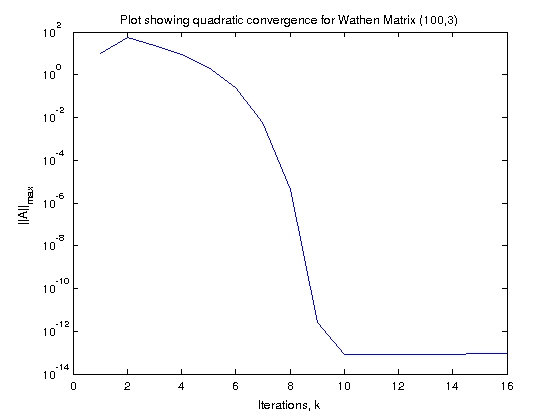
\includegraphics[scale=0.67]{configI.png}
\caption{Logaritmic plot of of the max norm of the Wathen 3,100 matrix with iteration I}
\label{fig:convergence plot I}
\end{figure}
\end{center}

\begin{center}
\begin{figure}[h!]
\centering
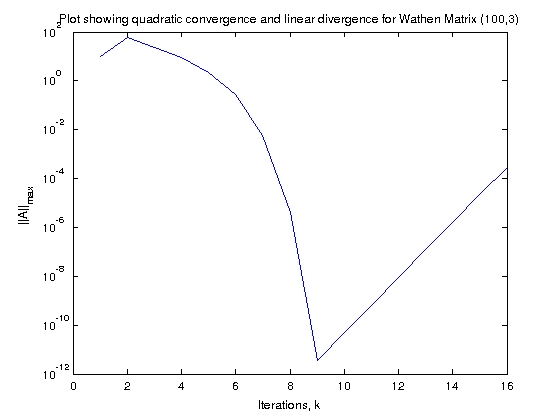
\includegraphics[scale=0.67]{configIII.png}
\caption{Logaritmic plot of of the max norm of the Wathen 3,100 matrix with iteration III}
\label{fig:convergence plot III}
\end{figure}
\end{center}




\begin{table}
\begin{center}
\label{Table: Wathen 100,3}

\begin{tabular}{| l | l | l | }

	\hline
	\multicolumn{3}{|c|}{Wathen Matrix 3,100}  \\
	\hline
	   & Implementation I & Implementation III \\
	k & $\parallel \Sigma^{1/2} - A_{k}\parallel_{\text{max}}$ & $\parallel \Sigma^{1/2} - A_{k}\parallel_{\text{max}}$  \\	
	\hline
	0 & 9.8425 & 9.8425  \\
	1 & 59.4301& 59.4301  \\
	2 & 25.2791& 25.2791   \\
	3 & 9.0880& 9.0880  \\
	4 & 2.3227& 2.3227  \\
	5 & 0.2889& 0.2889  \\
	6 & 0.0069& 0.0069  \\
	7 & 4.7293e-6& 4.7293e-6  \\
	8 & 3.7786e-10& 2.97183-12  \\
	9 & 1.5361e-8& 1.9995e-13  \\
	10& 6.4915e-7 & 1.9995e-13 \\ 
	11& 2.8050e-5 & \\
	\hline
	
\end{tabular}
\end{center}
\caption{Error of Wathen Matrix 100,3}
\end{table}

\begin{table}
\begin{center}
\label{Table: Wathen 10,3}
\begin{tabular}{| l | l | l | }

	\hline
	\multicolumn{3}{|c|}{Wathen Matrix 3,10}  \\
	\hline
	   & Implementation I & Implementation III \\
	k & $\parallel \Sigma^{1/2} - A_{k}\parallel_{\text{max}}$ & $\parallel \Sigma^{1/2} - A_{k}\parallel_{\text{max}}$  \\	
	\hline
	0 & 9.5764 & 9.5764 \\
	1 & 56.4823& 56.4823  \\
	2 & 23.9371& 23.9371   \\
	3 & 8.5418& 8.5418 \\
	4 & 2.1501& 2.1501  \\
	5 & 0.2574& 0.2574  \\
	6 & 0.0055& 0.0055  \\
	7 & 2.8432e-6& 2.8432e-6  \\
	8 & 8.1712e-13& 8.1357e-13  \\
	9 & 2.8479e-11& 2.6645e-14  \\
	10& 2.1642e-10 & 2.75e-14 \\ 
	11& 1.6469e-9 & 2.8422e-14\\
	12& & 2.8422e-14 \\
	\hline
	
\end{tabular}
\caption{Error of Wathen Matrix 10,3}
\end{center}
\end{table}


\begin{table}
\begin{center}
\label{Table: A5}
\begin{tabular}{| l | l | l | }

	\hline
	\multicolumn{3}{|c|}{Matrix A, n=5}  \\
	\hline
	   & Implementation I & Implementation III \\
	k & $\parallel \Sigma^{1/2} - A_{k}\parallel_{\text{max}}$ & $\parallel \Sigma^{1/2} - A_{k}\parallel_{\text{max}}$  \\	
	\hline
	0 &  5.8751& 5.8751 \\
	1 & 19.4577& 19.4577  \\
	2 & 7.4094& 7.4094   \\
	3 & 2.0943& 2.0943 \\
	4 & 0.3010& 0.3010  \\
	5 & 0.0093& 0.0093  \\
	6 & 1.1720e-5& 1.1720e-5  \\
	7 & 2.0964e-11& 2.0965e-5  \\
	8 & 3.2196e-15& 3.5527e-15 \\
	9 & 2.6645e-15& 2.6645e-15  \\
	10& 3.8858e-15 & 2.6645e-15\\ 
	11& 4.7740e-15 & 3.5527e-15\\
	12&5.3291e-15 & 3.5527e-15 \\
	13&5.8842e-15 &3.5527e-15 \\
	14& &3.5527e-15\\
	15& & 3.5527e-15 \\
	16& & 3.5527e-15 \\
	17& &4.4409e-15\\
	18& & 5.3291e-15\\
	19& &5.3291e-15 \\
	\hline
	
\end{tabular}
\caption{Error of Matrix A, n=5}
\end{center}
\end{table}

\begin{table}
\begin{center}
\label{Table: A10}
\begin{tabular}{| l | l | l | }

	\hline
	\multicolumn{3}{|c|}{Matrix A, n=10}  \\
	\hline
	   & Implementation I & Implementation III \\
	k & $\parallel \Sigma^{1/2} - A_{k}\parallel_{\text{max}}$ & $\parallel \Sigma^{1/2} - A_{k}\parallel_{\text{max}}$  \\	
	\hline
	0 &  12.6236& 12.6236 \\
	1 & 88.1618& 88.1618  \\
	2 & 38.6390& 38.6390   \\
	3 & 14.7314& 14.7314 \\
	4 & 4.1496& 4.1496 \\
	5 & 0.5961& 0.5961  \\
	6 & 0.0183& 0.0183  \\
	7 & 2.2952e-5& 2.2952e-5 \\
	8 & 4.6752e-11& 4.6724e-11 \\
	9 & 7.8826e-14& 8.8818e-15  \\
	10& 2.0961e-13& 8.8818e-15\\ 
	11& 5.7188e-13&1.0658e-14\\
	12&1.5721e-12& 1.0658e-14 \\
	13&4.3441e-12 & \\

	\hline
	
\end{tabular}
\caption{Error of Matrix A, n=10}
\end{center}
\end{table}

\begin{table}
\begin{center}
\label{Table: A100}
\begin{tabular}{| l | l | l | }

	\hline
	\multicolumn{3}{|c|}{Matrix A, n=100}  \\
	\hline
	   & Implementation I & Implementation III \\
	k & $\parallel \Sigma^{1/2} - A_{k}\parallel_{\text{max}}$ & $\parallel \Sigma^{1/2} - A_{k}\parallel_{\text{max}}$  \\	
	\hline
	0 &  134.8165& 134.8165 \\
	1 & 9.8737e+3&  9.8737e+3\\
	2 & 4.8742e+3&  4.8742e+3  \\
	3 & 2.3754e+3& 2.3754e+3 \\
	4 & 1.1279e+3& 1.1279e+3 \\
	5 & 507.9627& 507.9627  \\
	6 & 204.9391& 204.9391  \\
	7 & 65.3699& 65.3699 \\
	8 & 12.3950& 12.3950 \\
	9 & 0.7211& 0.7211  \\
	10& 0.0032& 0.0032\\ 
	11& 5.1975e-7&8.5515e-8\\
	12&1.1778e-5& 3.2685e-13 \\
	13&3.4155e-4 & 3.4106e-13 \\
	14&0.0099& 3.5527e-13\\
	15&0.2842 & 3.8369e-13\\
	16& 8.1845 & 4.6896e-13\\
	17& & 5.5422e-13\\
	18& & 6.3949e-13\\

	\hline
	
\end{tabular}
\caption{Error of Matrix A, n=100}
\end{center}
\end{table}

\begin{table}
\begin{center}
\label{Table: A1000}
\begin{tabular}{| l | l | l | }

	\hline
	\multicolumn{3}{|c|}{Matrix A, n=1000}  \\
	\hline
	   & Implementation I & Implementation III \\
	k & $\parallel \Sigma^{1/2} - A_{k}\parallel_{\text{max}}$ & $\parallel \Sigma^{1/2} - A_{k}\parallel_{\text{max}}$  \\	
	\hline
	0 & 1.3571e+3 & 1.3571e+3\\
	1& 9.9873e+5 & 9.9873e+5 \\
	2 &  4.9873e+5& 4.9837e+5 \\
	3 & 2.4873e+5&  2.4873e+5\\
	4 & 1.2373e+5&  1.2373e+5  \\
	5 & 6.1237e+4& 6.1237e+4\\
	6 & 2.9998e+4& 2.9998e+4 \\
	7 & 1.4394e+4& 1.4394e+4 \\
	8 & 6.6221e+3& 6.6221e+3  \\
	9 & 2.7936e+3& 2.7936e+3 \\
	10 & 981.1362& 981.1362 \\
	11 & 230.5792& 230.5792 \\
	12& 21.9698& 21.9698\\ 
	13& 9.9607&0.2756\\
	14&2.4619e+3& 5.6816e-5 \\
	15&6.3549e+5& 1.5234e-11 \\
	16& & 1.3870e-11\\
	17& & 1.5461e-11\\
	18& & 2.0464e-11\\
	
	\hline
	
\end{tabular}
\caption{Error of Matrix A, n=1000}
\end{center}
\end{table}


\begin{table}
\label{Table: Kondisjons tall}
\begin{center}
\begin{tabular}{| l | l | }

	
	\hline
	Matrix & Condtition number, $\kappa$\\	
	\hline
	A5 & 122484  \\
	A10 & 43,1690 \\
	A100 &3.3465e+10  \\
	A1000 & 3.6867e+10 \\
	W10 & 209.0646 \\
	W100 & 994.4419 \\
	
	\hline
	
\end{tabular}
\caption{Condition number of the matrices}
\end{center}
\end{table}



%\bibliosub
\end{document}